\section{平均码长}
\label{sec:lossless-average-length}

Kraft–McMillan不等式说明码长不能都很短：给一个符号分配短码字，就占去了$[0,1)$中一段长区间，留给其他符号的空间随之变小。现在把信源的概率加进来，问：在唯一可译的要求下，平均码长$L(c)$最小能到多少？

\paragraph{熵与自信息}
回答要用到第~\ref{chap:information-measures}章的两个量，这里按本部分的约定以$2$为底重新写出。符号$x$的自信息是$-\log_2p(x)$，单位为bit；信源的熵是自信息的平均，
\begin{equation}
 H(X)=-\sum_{x\in\mathcal{X}}p(x)\log_2p(x).
 \label{eq:lossless-entropy}
\end{equation}
第~\ref{chap:information-measures}章以自然对数计量，单位为nat；以nat计的熵除以$\ln2$，就得到这里以bit计的值。熵是“平均要问几个是非题才能确定结果”：若$p$是均匀分布，$\lvert\mathcal{X}\rvert=2^k$，则恰好需要$k$个是非题，此时$H(X)=k$。

贯穿例的四项自信息为
\[
 \begin{gathered}
 -\log_2 0.4=1.322,\qquad -\log_2 0.3=1.737,\\
 -\log_2 0.2=2.322,\qquad -\log_2 0.1=3.322 ,
 \end{gathered}
\]
按概率加权，
\[
 H(X)=0.4\times1.322+0.3\times1.737+0.2\times2.322+0.1\times3.322=1.846 .
\]

另一个工具是第~\ref{chap:distribution-comparison}章的KL散度。对$\mathcal{X}$上的两个概率质量函数$p$与$r$，若$r(x)>0$对每个$x$成立，
\[
 D_{\mathrm{KL}}(p\Vert r)=\sum_{x\in\mathcal{X}}p(x)\log_2\frac{p(x)}{r(x)}\geq0 ,
\]
等号当且仅当$p=r$。以$2$为底只是把以nat计的值除以$\ln2$，非负性和等号条件不变。

\paragraph{理想码长}
若码长可以取任意正实数，把$\ell(x)$取为$-\log_2p(x)$，Kraft和恰好是
\[
 \sum_x2^{\log_2p(x)}=\sum_xp(x)=1 ,
\]
平均码长恰好是$H(X)$。所以熵是“理想码长”下的平均码长：每个符号的码长等于它的自信息。下面的定理说明，任何唯一可译码都不能比这更短，而整数码长最多比它多出不到一位。

\begin{theorem}[平均码长的熵界]
\label{thm:lossless-entropy-bound}
设信源$X$取值于有限字母表$\mathcal{X}$，$\lvert\mathcal{X}\rvert\geq2$，且$p(x)>0$对每个$x$成立。
\begin{enumerate}
 \item 任何二进制唯一可译码$c$满足
 \begin{equation}
  L(c)\geq H(X),
  \label{eq:lossless-lower-bound}
 \end{equation}
 等号成立当且仅当对每个$x$都有$\ell(x)=-\log_2p(x)$。
 \item 取码长
 \begin{equation}
  \ell(x)=\bigl\lceil-\log_2p(x)\bigr\rceil ,
  \label{eq:lossless-shannon-length}
 \end{equation}
 存在具有这些码长的二进制前缀码，其平均码长满足
 \begin{equation}
  H(X)\leq L(c)<H(X)+1 .
  \label{eq:lossless-upper-bound}
 \end{equation}
\end{enumerate}
\end{theorem}

\begin{proof}
先证第一部分。记$K=\sum_x2^{-\ell(x)}$，由McMillan不等式（定理~\ref{thm:lossless-mcmillan}），$0<K\leq1$。用码长定义一个概率质量函数
\[
 r(x)=\frac{2^{-\ell(x)}}{K},\qquad x\in\mathcal{X},
\]
它的各项为正、和为$1$。由此$\ell(x)=-\log_2r(x)-\log_2K$。代入平均码长与熵之差，
\[
 \begin{aligned}
 L(c)-H(X)&=\sum_xp(x)\ell(x)+\sum_xp(x)\log_2p(x)\\
 &=\sum_xp(x)\log_2\frac{p(x)}{r(x)}-\log_2K .
 \end{aligned}
\]
第一项是$D_{\mathrm{KL}}(p\Vert r)$，非负；$K\leq1$使第二项$-\log_2K\geq0$。所以
\[
 L(c)-H(X)=D_{\mathrm{KL}}(p\Vert r)+\log_2\frac1K\geq0 .
\]
等号要求两项同时为零，即$K=1$且$r=p$，也就是$2^{-\ell(x)}=p(x)$对每个$x$成立。反过来，若$\ell(x)=-\log_2p(x)$，则$L(c)=H(X)$。

再证第二部分。由$\lvert\mathcal{X}\rvert\geq2$且各概率为正，每个$p(x)<1$，所以$-\log_2p(x)>0$，式~\eqref{eq:lossless-shannon-length}给出的$\ell(x)$都是正整数。上取整满足$\ell(x)\geq-\log_2p(x)$，即$2^{-\ell(x)}\leq p(x)$，求和得
\[
 \sum_x2^{-\ell(x)}\leq\sum_xp(x)=1 .
\]
由定理~\ref{thm:lossless-kraft}，存在具有这些码长的前缀码。又因为$\ell(x)<-\log_2p(x)+1$，乘以$p(x)$求和，
\[
 L(c)<\sum_xp(x)\bigl(-\log_2p(x)\bigr)+1=H(X)+1 .
\]
左边的不等号由第一部分得到，因为前缀码是唯一可译码。
\end{proof}

证明把$L(c)-H(X)$拆成两部分，它们分别说明码长损失从哪里来。$D_{\mathrm{KL}}(p\Vert r)$衡量码长所“暗含”的概率$r$与真实概率$p$的差距：码长$\ell(x)$相当于假定$x$的概率是$2^{-\ell(x)}$。$\log_2(1/K)$衡量Kraft不等式没有取等号所浪费的空间，即$[0,1)$中没有被码字占用的部分。

用贯穿例检验这一分解。第~\ref{sec:lossless-model}节的码长$1,2,3,3$满足$K=1$，第二项为零，暗含的概率是
\[
 r=\bigl(\tfrac12,\tfrac14,\tfrac18,\tfrac18\bigr),
\]
冗余$1.9-1.846=0.054$全部来自$D_{\mathrm{KL}}(p\Vert r)=0.054$：它把$a$的概率当成$0.5$、把$d$的概率当成$0.125$，与真实的$0.4$和$0.1$有偏差。下文的Shannon码长$2,2,3,4$给出$K=11/16$，浪费的空间贡献
\[
 \log_2\frac{16}{11}=0.541,
\]
暗含的概率$r=(4,4,2,1)/11$与$p$很接近，KL散度只有$0.013$。两项相加为$0.554$，正是它的冗余$2.4-1.846$。Shannon码的损失几乎全在没有用满的Kraft和上。

按式~\eqref{eq:lossless-shannon-length}取码长并按定理~\ref{thm:lossless-kraft}的方法分配码字，得到的码称为\term{Shannon码}（Shannon code）。平均码长与熵之差$L(c)-H(X)$称为码的\term{冗余}（redundancy）。

\paragraph{贯穿例}
贯穿例中$p(x)$都小于$1$，定理适用。Shannon码长为
\[
 \lceil1.322\rceil=2,\quad\lceil1.737\rceil=2,\quad\lceil2.322\rceil=3,\quad\lceil3.322\rceil=4 ,
\]
Kraft和为$11/16$，码字由图~\ref{fig:lossless-kraft-intervals}第二行给出。平均码长为
\[
 L=0.4\times2+0.3\times2+0.2\times3+0.1\times4=2.4 ,
\]
确实落在$[1.846,\,2.846)$中。可是它比两位定长码还长。第~\ref{sec:lossless-model}节的码$0,10,110,111$平均只要$1.9$位，冗余为$0.054$。式~\eqref{eq:lossless-upper-bound}只保证冗余小于$1$，并不说明Shannon码是好的码；平均码长最短的码由第~\ref{sec:lossless-huffman}小节构造。

\paragraph{冗余是平均量}
冗余小于$1$说的是平均。逐个符号看，码长与自信息之差$\ell(x)+\log_2p(x)$各不相同，图~\ref{fig:lossless-length-vs-selfinfo}把它们画在一起。对Shannon码，这个差在$[0,1)$中，四个符号分别是
\[
 0.678,\quad 0.263,\quad 0.678,\quad 0.678 .
\]
对码$0,10,110,111$，四个差分别是
\[
 -0.322,\quad 0.263,\quad 0.678,\quad -0.322 ,
\]
其中$a$与$d$的码长比自信息还短。所以“整数码长带来不到一位的冗余”不是说每条消息都比它的自信息长同样多：个别符号可以比自信息短，个别可以长将近一位，下界$L\geq H$只约束加权平均。

\begin{BookInlineFigure}
 \centering
 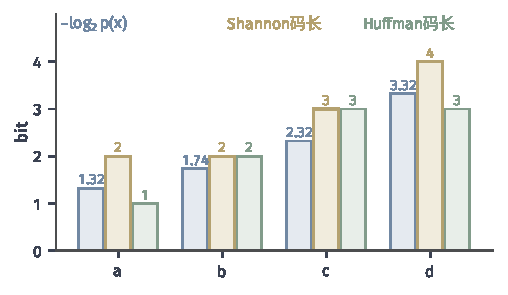
\includegraphics[width=86mm]{figures/07-probability/05-source-coding/matplotlib/lossless-length-vs-selfinfo/figure.pdf}
 \caption{贯穿例中每个符号的自信息$-\log_2p(x)$（蓝）、Shannon码长$\lceil-\log_2p(x)\rceil$（黄）和第~\ref{sec:lossless-model}节码表的码长（绿）。Shannon码长总不小于自信息；后一张码表中$a$与$d$的码长小于自信息，平均码长$1.9$却仍不小于熵$1.846$。}
 \label{fig:lossless-length-vs-selfinfo}
\end{BookInlineFigure}

\paragraph{冗余可以接近一位}
上界中的$+1$不能改进成更小的常数。取二元信源$\mathcal{X}=\{0,1\}$，$p(1)=\theta$。任何唯一可译码的码字至少一位，所以平均码长至少为$1$；而熵
\[
 H(\theta)=-\theta\log_2\theta-(1-\theta)\log_2(1-\theta)
\]
在$\theta\to0$时趋于$0$。$\theta=0.1$时$H=0.469$，最优码仍要$1$位，冗余$0.531$；$\theta$越小，冗余越接近$1$。图~\ref{fig:lossless-binary-bounds}画出这一情形。问题在于每个符号至少要花一位：概率极不均匀时，一个符号所含的信息远少于一位，逐符号编码无法用“半位”来记录它。第~\ref{sec:lossless-block-limits}节把多个符号合成一块编码，正是为了把这一位摊到许多符号上。

\begin{BookInlineFigure}
 \centering
 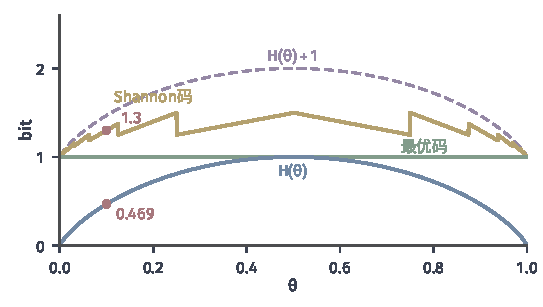
\includegraphics[width=92mm]{figures/07-probability/05-source-coding/matplotlib/lossless-binary-bounds/figure.pdf}
 \caption{二元信源$p(1)=\theta$的逐符号编码。蓝线为熵$H(\theta)$，紫色虚线为上界$H(\theta)+1$，黄线为Shannon码的平均码长，绿线为最优码的平均码长$1$。红点标出$\theta=0.1$处的$H=0.469$与Shannon码长$1.3$。黄线在$\theta=1/2$处另有一个孤立的取值$1$，图中未画出。}
 \label{fig:lossless-binary-bounds}
\end{BookInlineFigure}

\paragraph{确定源}
定理~\ref{thm:lossless-entropy-bound}要求至少两个符号有正概率。若只有一个符号$x_0$，$p(x_0)=1$，则$H(X)=0$，式~\eqref{eq:lossless-shannon-length}给出的码长是$0$，即空码字。这时要看解码器知道什么。

若消息长度$n$事先约定，接收方知道消息必定是$x_0x_0\cdots x_0$（$n$个），什么都不必发送，平均码长为$0$，等于熵。若长度没有约定，空码字无法告诉接收方发出了几个符号：$n=1$和$n=5$的消息都编成空串。由第~\ref{sec:lossless-decodability}节，唯一可译码不含空码字，每个符号至少一位，平均码长至少为$1$；另一种做法是单独传送长度$n$，所需位数随$n$增长，但这已不是逐符号编码的问题。所以确定源的“零码长”只在长度已知时成立，这正是定理把它排除在外的原因。
